% Compile with XeLaTeX
\documentclass[aspectratio=169,11pt]{ctexbeamer}

\usetheme{Madrid}
\usecolortheme{default}
\usefonttheme[onlymath]{serif}
\setbeamertemplate{navigation symbols}{}
\setbeamertemplate{footline}[frame number]

\usepackage{amsmath,amssymb,bm}
\usepackage{booktabs}
\usepackage{array}
\usepackage{graphicx}
\usepackage{hyperref}

\title{Representation-Dependent Recoverability in Quantum Compilation}
\subtitle{Fourier-layer separation, semantic UCC artifact, and evidence chain}
\author{杨锦泽}
\date{\today}

\newcommand{\basis}{\mathcal{L}_B}
\newcommand{\uccpipe}{\mathcal{P}_{\mathrm{ucc}}}
\newcommand{\cost}{\kappa}
\newcommand{\flatclass}{\mathfrak{F}^{\mathrm{fl}}_{w,b,\rho}}
\newcommand{\lcclass}{\mathfrak{F}^{\mathrm{lc}}_{w,b,\rho}}
\newcommand{\sem}[1]{\mathcal{U}(#1)}
\newcommand{\pg}{\operatorname{pg}_B}

\begin{document}

\begin{frame}
  \titlepage
\end{frame}

\begin{frame}{本报告的目标}
  当前论文已经收束成一条主线：

  \begin{center}
    \Large
    \textbf{量子电路 lowering 保留酉语义，}\\
    \textbf{但可能改变结构的可恢复性。}
  \end{center}

  \vspace{0.8em}
  本报告按论文结构展开：

  \begin{enumerate}
    \item 问题：representation-dependent recoverability gap
    \item 定理：Fourier-layer recoverability separation
    \item artifact：semantic UCC controller 怎样实现该原则
    \item 证据链：separation、ablation、resource consequence、scope
    \item 边界：restricted class、外部 baseline、claim scope
  \end{enumerate}
\end{frame}

\tableofcontents

\section{核心问题}

\begin{frame}{电路语义与电路表示}
  一个量子电路可以看成酉算子：
  \[
    \sem{C}\in U(2^n).
  \]

  编译器实际操作的是某种表示：
  \[
    C=(g_1,g_2,\ldots,g_m).
  \]

  正确编译要求：
  \[
    \sem{C}=\sem{C'}.
  \]

  论文关注的额外问题：
  \[
    \text{same unitary}
    \quad\Longrightarrow?\quad
    \text{same recoverable structure}.
  \]

  关键观察：
  \begin{center}
    \textbf{酉语义相同，不保证优化证据在当前表示中仍然低成本可恢复。}
  \end{center}
\end{frame}

\begin{frame}{lower-then-optimize 的表示风险}
  常见流水线：
  \[
    C
    \xrightarrow{\basis}
    \basis(C)
    \xrightarrow{\text{flat optimization}}
    C_{\mathrm{out}}.
  \]

  lowering 是语义保持的：
  \[
    \sem{C}=\sem{\basis(C)}.
  \]

  结构保持没有自动成立。结构化电路中的对象：
  \[
    B^r,\qquad U U^\dagger,\qquad H D^r H,\qquad U M U^\dagger,
  \]
  在 target-basis stream 中可能变成很长的局部门序列。

  \begin{center}
    \textbf{问题从“能否等价变换”变成“还能否认证原来的全局结构”。}
  \end{center}
\end{frame}

\begin{frame}{Recoverability Gap}
  论文定义的核心现象：

  \begin{center}
    \Large
    \textbf{representation-dependent recoverability gap}
  \end{center}

  设 $\mathcal{T}_K(C)$ 是 bounded semantic terms，$\mathfrak{A}_w$ 是 bounded flat recovery class。

  \[
  \mathrm{Gap}^{K,w}_{\mathrm{rep}}(C)
  =
  \inf_{A\in\mathfrak{A}_w}\cost(A(\basis(C)))
  -
  \inf_{T\in\mathcal{T}_K(C)}\cost(\basis(T)).
  \]

  直观含义：
  \[
    \text{flat lowered stream sees local fragments;}
    \qquad
    \text{semantic terms still name global objects.}
  \]
\end{frame}

\begin{frame}{两个 operational regimes}
  论文区分两个 regime：

  \begin{block}{1. Structural separation}
    semantic representation 暴露全局聚合机会；restricted flat compiler 在 lowering 后无法从局部证据恢复。
  \end{block}

  \vspace{0.5em}

  \begin{block}{2. Recoverability parity}
    semantic lifting 防止 baseline UCC regression，并恢复到强 flat baseline 的输出质量。
  \end{block}

  \vspace{0.8em}
  当前论文的主定理属于第一类：
  \[
    H_{\Lambda}D_m(\bm{\theta})^rH_{\Lambda}
    \quad\leadsto\quad
    \Omega(rm)\ \text{vs}\ O(m).
  \]

  mirrored/conjugation 结果属于第二类。
\end{frame}

\begin{frame}{UCC 在论文中的角色}
  UCC 在论文中作为 artifact 和 diagnostic testbed：

  \begin{itemize}
    \item 默认 UCC 路径具有多前端、多后端的组合性
    \item 这种组合性也可能导致结构化电路 regression
    \item semantic UCC artifact 用来验证 representation principle
  \end{itemize}

  \vspace{0.8em}
  当前论文的对象：

  \begin{center}
    \textbf{recoverability principle}
  \end{center}

  \vspace{0.4em}
  UCC 的角色：

  \begin{center}
    \textbf{可复现实验载体，而非最终科学对象。}
  \end{center}
\end{frame}

\section{Semantic UCC Artifact}

\begin{frame}{semantic UCC controller}
  semantic UCC artifact 改变 UCC flow 的六个位置：

  \begin{enumerate}
    \item lowering 前做 bounded structural simplification
    \item 将合适子电路 lift 到 bounded semantic term algebra
    \item 用 conservative cost selection 防止 regression
    \item 对 all-to-all Qiskit-native case 使用 source-level short circuit
    \item 后端感知 portfolio 只在必要时扩展
    \item 对 semantic references 和 repeated-run block selections 做 cache
  \end{enumerate}

  \vspace{0.6em}
  核心控制逻辑：
  \[
    \text{recognize structure}
    \to
    \text{compare semantic candidates}
    \to
    \text{late materialization}.
  \]
\end{frame}

\begin{frame}{主定理图：表示差距}
  \centering
  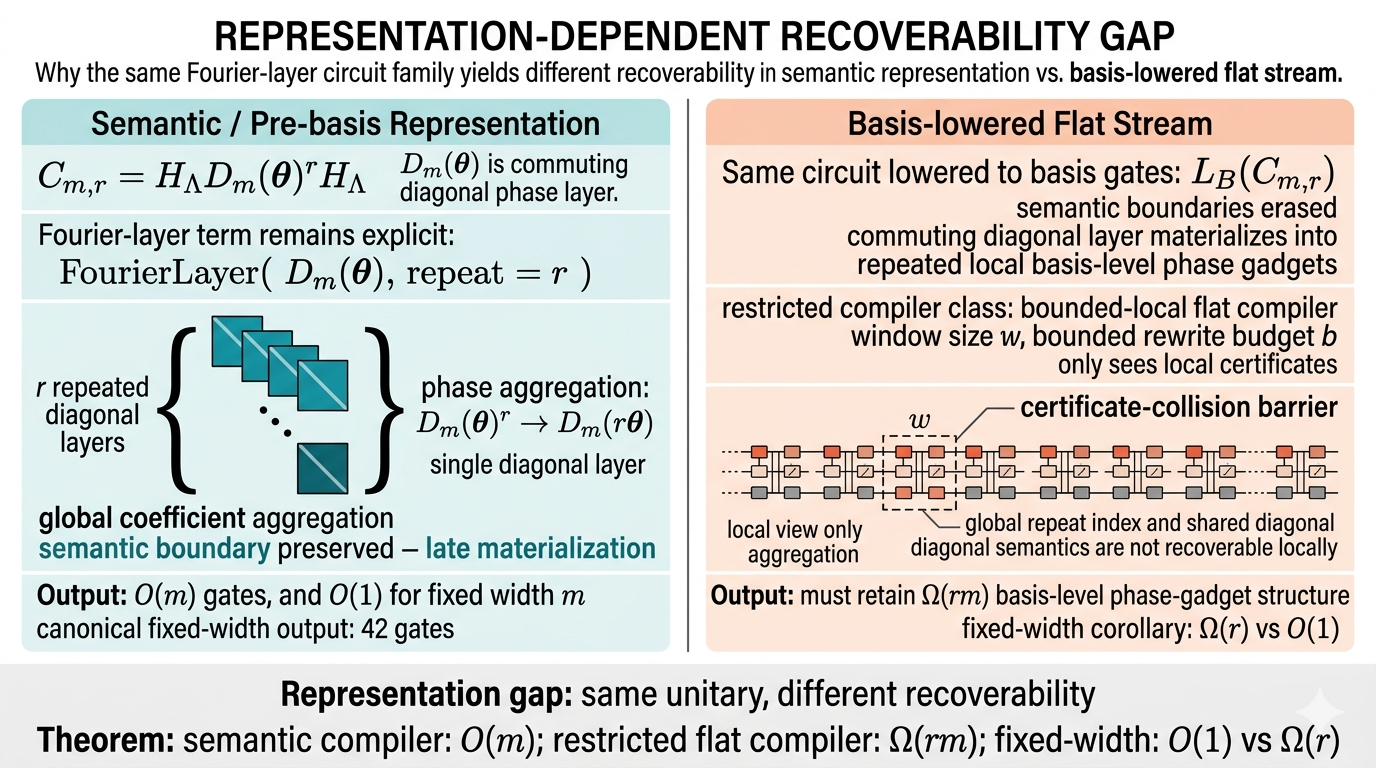
\includegraphics[
    width=0.92\linewidth,
    height=0.72\textheight,
    keepaspectratio
  ]{../Graph Materials/conceptual_theorem_figure.png}

  \vspace{0.4em}
  \small
  同一个 unitary 在 semantic 表示中保留可聚合结构；在 basis-lowered flat stream 中只剩局部证据。
\end{frame}

\begin{frame}{semantic term algebra}
  artifact 使用小型层次化 term algebra：
  \[
  T ::= \mathrm{Leaf}(C)
  \mid \mathrm{Node}(v)
  \mid T_1\circ T_2
  \mid T^r
  \mid \mathrm{Conj}(U,M)
  \mid \mathrm{Fourier}(F_1,\ldots,F_\ell)
  \mid \mathrm{Mirror}(D,S).
  \]

  代码层对应：
  \begin{itemize}
    \item \texttt{\_SemanticRepeatTerm}
    \item \texttt{\_SemanticConjugationTerm}
    \item \texttt{\_SemanticFourierLayerTerm}
    \item \texttt{\_SemanticMirroredSelfInverseTerm}
  \end{itemize}

  作用：
  \begin{center}
    \textbf{把全局结构作为编译和 cache 的单位，而非只作为 flat gate stream。}
  \end{center}
\end{frame}

\begin{frame}{Fourier-layer path}
  对 phase-heavy circuit：
  \[
  \begin{aligned}
    \text{diagonal phase span}
    &\to
    \text{aggregate equal signatures} \\
    &\to
    \text{phase-ladder node}
    \to
    \text{Fourier-layer term}
    \to
    \text{late lowering}.
  \end{aligned}
  \]

  关键点：
  \[
    CP(\theta)
    \leadsto
    RZ(\theta/2)\,CX\,RZ(-\theta/2)\,CX\,RZ(\theta/2).
  \]

  如果先展开 $r$ 次，再尝试恢复相位聚合，局部证据会分散。

  如果先保留 phase term：
  \[
    (P,\theta)^r\mapsto(P,r\theta).
  \]
\end{frame}

\begin{frame}{Repeated-run path}
  对 repeated-run family：
  \[
    C=P\circ B^r\circ S.
  \]

  artifact 避免先 materialize 多个完整大候选：

  \begin{enumerate}
    \item 编译 prefix $P$ 和 suffix $S$
    \item 为 block $B$ 生成 bounded candidate set $\{B_i\}$
    \item 用 projected metrics 估计 $P\circ B_i^r\circ S$
    \item 只 materialize winning block
  \end{enumerate}

  这样 repeated structure 与实现策略一致：
  \[
    \text{compare block-level semantics before full expansion}.
  \]
\end{frame}

\section{Fourier-Layer Theorem}

\begin{frame}{theorem family}
  定义 commuting diagonal phase layer：
  \[
    D_m(\bm{\theta})
    =
    \prod_{j=1}^m
    \exp(-i\theta_jP_j/2),
    \qquad
    [P_i,P_j]=0.
  \]

  Fourier-layer witness family：
  \[
    C_{m,r}
    =
    H_{\Lambda}D_m(\bm{\theta})^rH_{\Lambda}.
  \]

  这个 family 的特点：
  \begin{itemize}
    \item 没有 $U U^\dagger$ inverse cancellation
    \item 唯一关键机会是 commuting coefficient aggregation
    \item 固定宽度 $m=m_0$ 时，semantic side 输出常数大小
  \end{itemize}
\end{frame}

\begin{frame}{restricted flat compiler class}
  flat compiler class 记为：
  \[
    \flatclass.
  \]

  它接收 fully basis-lowered stream：
  \[
    \basis(C_{m,r}).
  \]

  允许能力：
  \begin{itemize}
    \item radius-$w$ local windows
    \item at most $b$ bounded candidate rounds
    \item phase fusion 需要至多 $\rho$ 个 local witness windows
  \end{itemize}

  排除能力：
  \begin{itemize}
    \item global phase-polynomial reconstruction
    \item global ZX / stabilizer-phase lift
    \item commuting-diagonal Hamiltonian lift
  \end{itemize}
\end{frame}

\begin{frame}{semantic upper bound}
  semantic compiler 在 lowering 前保留：
  \[
    (P_j,\theta_j),\qquad j=1,\ldots,m.
  \]

  因为所有 $P_j$ commute：
  \[
  \begin{aligned}
  D_m(\bm{\theta})^r
  &=
  \left(
    \prod_{j=1}^{m}e^{-i\theta_jP_j/2}
  \right)^r \\
  &=
  \prod_{j=1}^{m}e^{-i(r\theta_j)P_j/2}.
  \end{aligned}
  \]

  term 层执行：
  \[
    (P_j,\theta_j)\mapsto(P_j,r\theta_j).
  \]

  每个 bounded-arity term lowering 一次：
  \[
    \pg(\basis(S(C_{m,r})))\le C m.
  \]
\end{frame}

\begin{frame}{flat lower bound intuition}
  lowering 后，第 $j$ 个 phase term 的第 $t$ 次出现记为：
  \[
    G_{j,t},\qquad
    j=1,\ldots,m,\quad t=1,\ldots,r.
  \]

  periodic separated lowering 假设：
  \[
    G_{j,t}\ \text{和}\ G_{j,t+1}
    \ \text{不落在同一个 radius-}w\text{ window 中}.
  \]

  interior certificates 重复出现：
  \[
    \mathrm{mult}
    \bigl(
      \mathrm{cert}(\partial,\basis(C_{m,r}))
    \bigr)
    =
    \Theta(r).
  \]

  含义：
  \begin{center}
    \textbf{局部窗口反复看到相同证据，无法唯一认证全局 phase aggregation。}
  \end{center}
\end{frame}

\begin{frame}{main theorem}
  \begin{block}{Fourier-layer recoverability separation}
    对
    \[
      C_{m,r}=H_{\Lambda}D_m(\bm{\theta})^rH_{\Lambda},
    \]
    若 $m>w$ 且满足 bounded arity、non-resonance、periodic separated lowering 和 bounded local recovery 假设，则对所有 $A\in\flatclass$：
    \[
      \pg(A(\basis(C_{m,r})))\ge c\,rm-O(m).
    \]
    同时存在 semantic compiler $S$：
    \[
      \pg(\basis(S(C_{m,r})))\le C m.
    \]
  \end{block}

  固定宽度 $m=m_0>w$：
  \[
    \Omega(r)\quad\text{vs}\quad O(1).
  \]
\end{frame}

\begin{frame}{theorem boundary}
  这个 theorem 是 restricted-class separation。

  它的含义：
  \[
    \text{bounded flat local recovery}
    \quad\text{vs}\quad
    \text{pre-basis semantic lift}.
  \]

  它的边界：
  \begin{itemize}
    \item 若编译器重建 global phase-polynomial IR，它属于 semantic side
    \item 若编译器重建 ZX 或 commuting-diagonal IR，它也属于 semantic side
    \item 外部 baseline 实验用于诊断 configured pipeline 属于哪一侧
  \end{itemize}

  因而 claim 不针对某个软件的永久能力上限。

  claim 是：
  \begin{center}
    \textbf{恢复 global diagonal object 是 closing the gap 的关键表示步骤。}
  \end{center}
\end{frame}

\section{Evidence Chain}

\begin{frame}{evidence chain}
  当前结果按证据链组织：

  \begin{enumerate}
    \item \textbf{Primary theorem witness}: canonical and generalized fixed-width $H D^r H$
    \item \textbf{External pipeline diagnostics}: Qiskit / PyZX / TKET
    \item \textbf{Causal ablation}: disable Fourier semantic path
    \item \textbf{Resource consequence}: semantic-first vs materialize-first
    \item \textbf{Natural-source controls}: QFT / AQFT / QPE / AE / QFT arithmetic
    \item \textbf{Secondary recoverability}: mirrored/conjugation parity recovery
  \end{enumerate}

  读法：
  \begin{center}
    \textbf{实验服务于 representation boundary 的验证，而非软件排名。}
  \end{center}
\end{frame}

\begin{frame}{primary witness: fixed-width Fourier-layer}
  \small
  \begin{tabular}{rrrr}
    \toprule
    Requested & \texttt{qiskit opt3} & PyZX pipeline & semantic UCC \\
    \midrule
    4k & 9{,}588 & 13{,}574 & 42 \\
    10k & 23{,}988 & 33{,}974 & 42 \\
    20k & 47{,}988 & 67{,}974 & 42 \\
    50k & timeout & timeout & 42 \\
    100k & timeout & timeout & 42 \\
    \bottomrule
  \end{tabular}

  \vspace{0.8em}
  TKET FullPeephole 在固定协议下从 4k 起 timeout。

  \vspace{0.8em}
  这张表对应 theorem 的 fixed-width corollary：
  \[
    \Omega(r)\quad\text{vs}\quad O(1).
  \]
\end{frame}

\begin{frame}{generalized witness suite}
  \small
  新数据把 canonical full-pair witness 扩成固定宽度参数化 suite：

  \vspace{0.4em}
  \begin{itemize}
    \item 主 suite 固定 $n=4$，用于测试 topology / angle / scale 轴
    \item 新增 full-pair width-axis stress 覆盖 $n=5,6$
    \item topology: chain / ring / sparse-0.5 / full-pair CP
    \item angle family: nonresonant seeded / QFT-dyadic / mixed-signed
    \item sizes: 4k / 10k / 20k / 50k
  \end{itemize}

  \vspace{0.6em}
  核心结果：
  \[
    \text{semantic UCC vs qiskit opt3:
    strict structural wins } 42/42.
  \]

  \vspace{0.4em}
  \texttt{qiskit opt3} 在 28 个 comparable points 完成，在 14 个 points timeout；
  semantic UCC 完成全部 42 个 comparable points。
\end{frame}

\begin{frame}{generalized witness: topology summary}
  \scriptsize
  \begin{tabular}{lrrrr}
    \toprule
    Topology & Points & Qiskit ok & Qiskit timeout & Semantic wins \\
    \midrule
    chain CP & 12 & 9 & 3 & 12/12 \\
    ring CP & 12 & 9 & 3 & 12/12 \\
    sparse CP 0.5 & 12 & 6 & 6 & 12/12 \\
    full-pair CP & 6 & 4 & 2 & 6/6 \\
    \midrule
    total & 42 & 28 & 14 & 42/42 \\
    \bottomrule
  \end{tabular}

  \vspace{0.8em}
  读法：
  \[
    \text{output depends on diagonal term structure, not on repetition count } r.
  \]

  \vspace{0.4em}
  full-pair CP 是 42-gate canonical case；chain/ring/sparse 给出同一原理的拓扑鲁棒性。
\end{frame}

\begin{frame}{width-axis external stress}
  \scriptsize
  \begin{tabular}{lrrrr}
    \toprule
    Case & semantic & \texttt{qiskit} & PyZX & TKET \\
    \midrule
    $n=5$, 4k & 65 & 11{,}711 & 14{,}640 & 30{,}369 \\
    $n=5$, 10k & 65 & 29{,}315 & 36{,}640 & timeout \\
    $n=6$, 4k & 93 & 12{,}108 & 15{,}321 & 33{,}881 \\
    $n=6$, 10k & 93 & 30{,}417 & 38{,}487 & timeout \\
    \bottomrule
  \end{tabular}

  \vspace{0.8em}
  \small
  解释：
  \begin{itemize}
    \item semantic output 随 diagonal term count 增长：$42 \to 65 \to 93$
    \item Qiskit 和 PyZX 在 configured bridge pipeline 中仍保持万级输出
    \item TKET 在 4k 完成但输出更大，在 10k timeout
  \end{itemize}

  \vspace{0.4em}
  这是一组 pipeline-specific diagnostic，用于定位 representation boundary。
\end{frame}

\begin{frame}{figure: Fourier-layer separation}
  \centering
  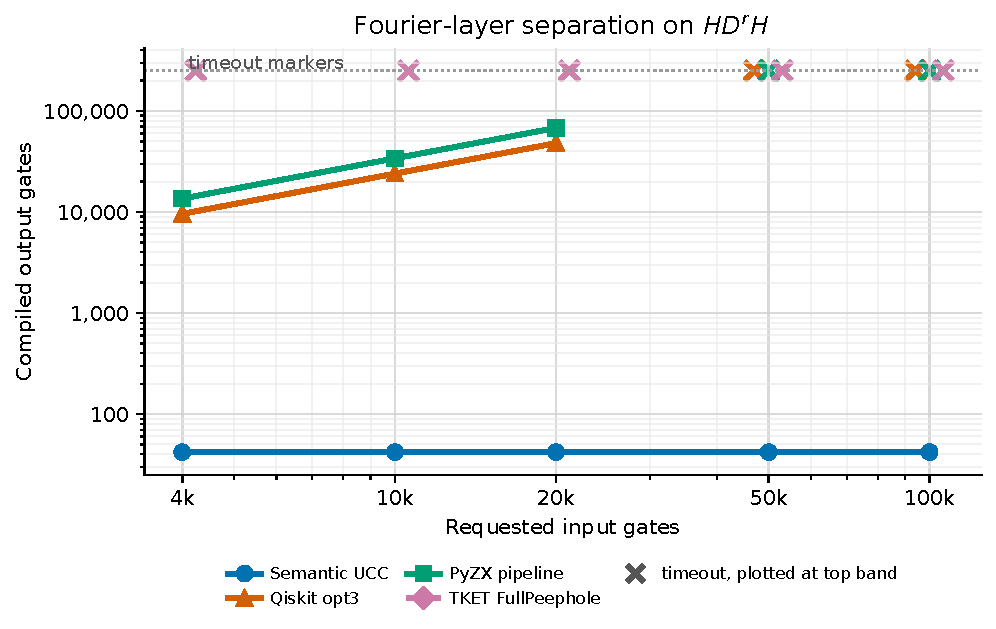
\includegraphics[
    width=0.92\linewidth,
    height=0.74\textheight,
    keepaspectratio
  ]{../Graph Materials/01_fourier_separation.pdf}

  \vspace{0.4em}
  \small
  semantic UCC 保持 $42$-gate canonical output；tested flat pipelines 增长或 timeout。
\end{frame}

\begin{frame}{causal ablation}
  \small
  \begin{tabular}{rrrr}
    \toprule
    Requested & Fourier-enabled UCC & no Fourier IR & \texttt{qiskit opt3} \\
    \midrule
    4k & 42 & timeout & 9{,}588 \\
    10k & 42 & timeout & 23{,}988 \\
    20k & timeout & timeout & timeout \\
    50k & 42 & timeout & timeout \\
    100k & 42 & timeout & timeout \\
    \bottomrule
  \end{tabular}

  \vspace{0.8em}
  机制结论：
  \[
    \text{Fourier semantic path disabled}
    \quad\Rightarrow\quad
    \text{completed constant recovery disappears}.
  \]

  20k row 所有方法 timeout，只作为 runtime caveat。
\end{frame}

\begin{frame}{figure: Fourier ablation}
  \centering
  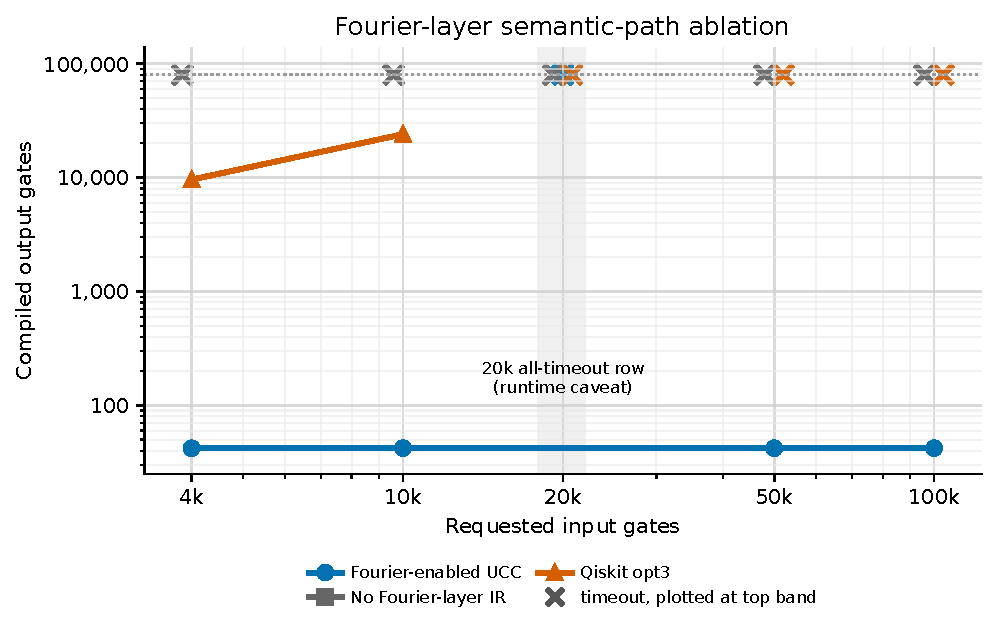
\includegraphics[
    width=0.92\linewidth,
    height=0.74\textheight,
    keepaspectratio
  ]{../Graph Materials/03_fourier_ablation.pdf}

  \vspace{0.4em}
  \small
  关掉 Fourier semantic path 后，完成的常数输出恢复消失；这把结果和机制绑定起来。
\end{frame}

\begin{frame}{resource consequence}
  对 fixed-width $H D^r H$，比较 semantic-first 与 materialize-first。

  \[
    T_{\epsilon}(R)=
    \left\lceil 3\log_2(1/\epsilon)\right\rceil R.
  \]

  \small
  \begin{tabular}{rrrr}
    \toprule
    Requested & semantic first & qiskit materialize first & no-Fourier UCC \\
    \midrule
    4k & 42 / 22 / 2{,}200 & 9{,}588 / 4{,}793 / 479{,}300 & 9{,}588 / 4{,}793 / 479{,}300 \\
    10k & 42 / 22 / 2{,}200 & 23{,}988 / 11{,}993 / 1{,}199{,}300 & timeout \\
    20k & 42 / 22 / 2{,}200 & 47{,}988 / 23{,}993 / 2{,}399{,}300 & timeout \\
    50k & 42 / 22 / 2{,}200 & timeout & timeout \\
    100k & 42 / 22 / 2{,}200 & timeout & timeout \\
    \bottomrule
  \end{tabular}

  \vspace{0.5em}
  每格为 gates / rotations / $T_{10^{-10}}$ proxy。
\end{frame}

\begin{frame}{figure: resource consequence}
  \centering
  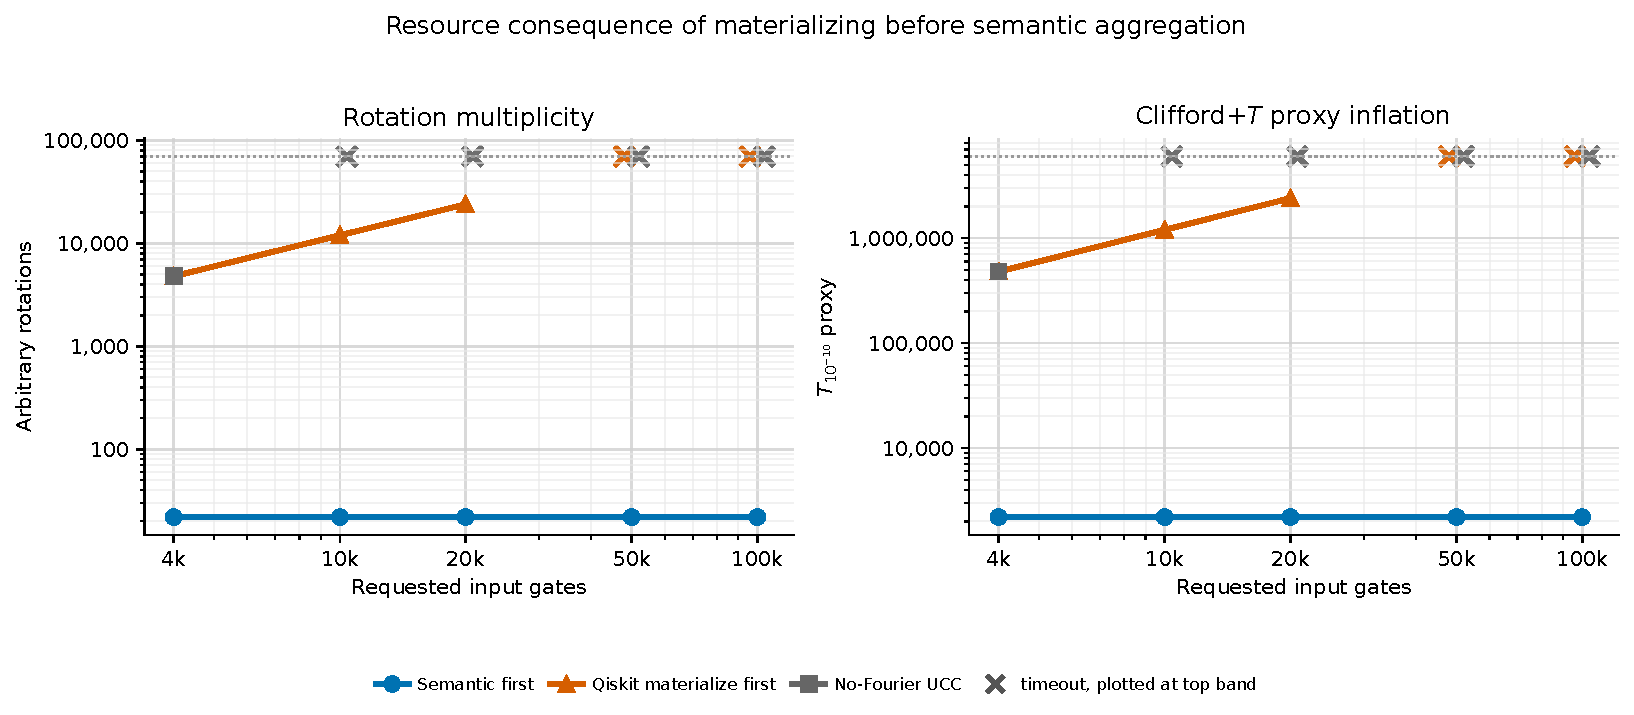
\includegraphics[
    width=0.92\linewidth,
    height=0.74\textheight,
    keepaspectratio
  ]{../Graph Materials/02_resource_consequence.pdf}

  \vspace{0.4em}
  \small
  semantic-first aggregation 让 resource estimator 看到常数数量的 rotation tasks。
\end{frame}

\begin{frame}{FTQC interpretation}
  在 FTQC pipeline 中，arbitrary rotations 通常进入 synthesis / resource estimation。

  两种顺序带来的输入规模不同：
  \[
    \text{semantic aggregation}
    \to
    \text{one aggregated coefficient}
    \to
    \text{synthesis estimate}.
  \]

  \[
    \text{basis materialization}
    \to
    \text{many separate rotations}
    \to
    \text{synthesis estimate}.
  \]

  当前 $T$ proxy 的作用：
  \begin{center}
    \textbf{展示 scaling consequence；精确最优 Clifford+$T$ count 属于后续 synthesis 问题。}
  \end{center}
\end{frame}

\begin{frame}{natural-source controls}
  这些 benchmark 连接 theorem witness 与自然算法来源。

  \small
  \begin{tabular}{lll}
    \toprule
    Source & semantic object & role \\
    \midrule
    QFT & Hadamard + controlled phase & repeat controls \\
    AQFT & truncated phase layer & approximate QFT control \\
    QPE & phase accumulation + inverse QFT & real and MQT QPE cases \\
    AE & Fourier-style phase accumulation & amplitude-estimation case \\
    Draper adder & QFT arithmetic & QFT arithmetic case \\
    \bottomrule
  \end{tabular}

  \vspace{0.8em}
  作用：
  \begin{center}
    \textbf{fixed-width witness 抽象的是自然算法中真实存在的 Fourier-layer object。}
  \end{center}
\end{frame}

\begin{frame}{official real instances}
  \small
  \begin{tabular}{lrrr}
    \toprule
    Instance & baseline UCC & semantic UCC & \texttt{qiskit opt3} \\
    \midrule
    \texttt{phase\_estimation\_real} & 471{,}819 & 166{,}805 & 166{,}805 \\
    \texttt{grover\_real} & 287{,}047 & 79{,}029 & 79{,}029 \\
    \texttt{qaoa\_real} & 167{,}833 & 36{,}512 & 36{,}512 \\
    \bottomrule
  \end{tabular}

  \vspace{0.8em}
  这些 case 的角色：
  \begin{itemize}
    \item 证明 semantic artifact 能修复真实 algorithm-family regression
    \item 输出质量恢复到 \texttt{qiskit opt3} parity
    \item 它们属于 recoverability parity evidence
  \end{itemize}
\end{frame}

\begin{frame}{figure: official real instances}
  \centering
  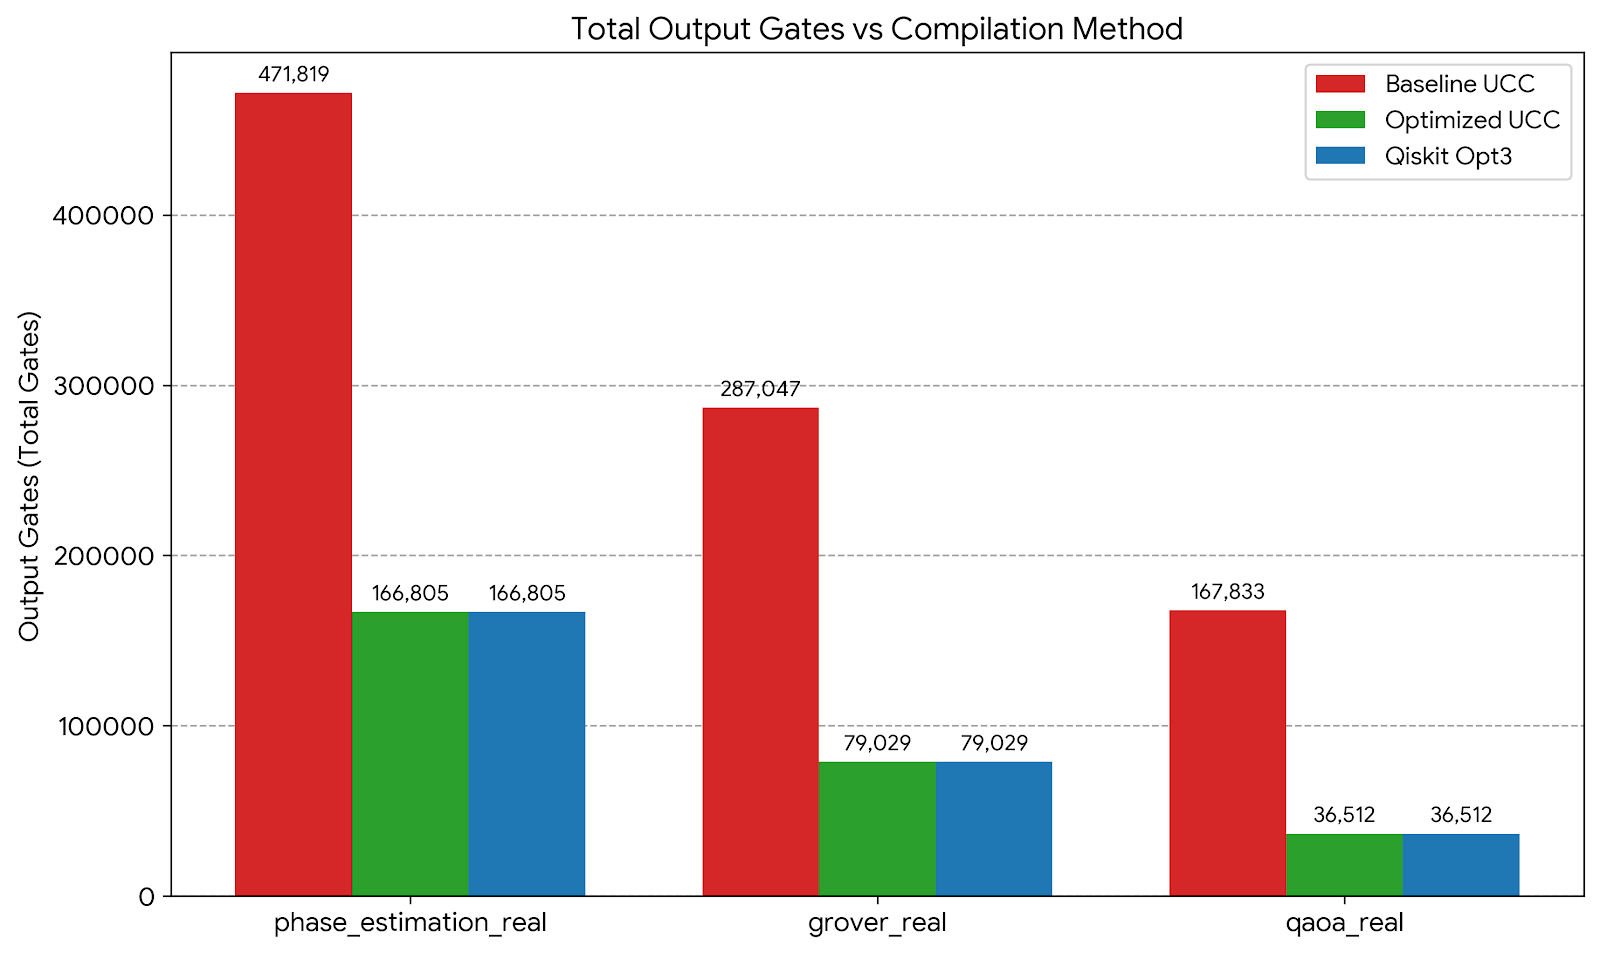
\includegraphics[
    width=0.92\linewidth,
    height=0.74\textheight,
    keepaspectratio
  ]{../PaperDraft/figures/real_instance_grouped_bar.png}

  \vspace{0.4em}
  \small
  semantic UCC 在三个 official real instances 上恢复到 \texttt{qiskit opt3} 输出质量。
\end{frame}

\begin{frame}{mirrored / conjugation family}
  \small
  \begin{tabular}{lrrr}
    \toprule
    Case & baseline UCC & semantic UCC & \texttt{qiskit opt3} \\
    \midrule
    \texttt{grover\_real} & 287{,}047 & 79{,}029 & 79{,}029 \\
    \texttt{mqt\_grover\_8} & 18{,}992 & 5{,}170 & 5{,}170 \\
    \texttt{mqt\_grover\_12} & 259{,}797 & 71{,}706 & 71{,}706 \\
    \texttt{mqt\_grover\_16} & 2{,}112{,}285 & 581{,}098 & 581{,}098 \\
    \texttt{grover\_mirrored\_100k} & 4{,}122{,}006 & 1{,}158{,}011 & 1{,}158{,}011 \\
    \bottomrule
  \end{tabular}

  \vspace{0.8em}
  解释：
  \begin{itemize}
    \item mirrored/conjugation 属于 secondary recoverability evidence
    \item 它证明 semantic lifting 是 anti-regression mechanism
    \item 强 flat compiler 能恢复 parity 时，论文按 parity evidence 处理
  \end{itemize}
\end{frame}

\section{Claim Boundary}

\begin{frame}{pass-ordering 质疑}
  质疑：
  \begin{center}
    \texttt{qiskit opt3} 表现更稳时，UCC 问题是否只是 pass ordering？
  \end{center}

  论文回答分两层：

  \begin{enumerate}
    \item UCCDefault regression 中，pass ordering 可以解释一部分
    \item fixed-width Fourier-layer separation 需要 global diagonal representation
  \end{enumerate}

  支撑点：
  \begin{itemize}
    \item $H D^r H$ 没有 inverse cancellation
    \item Qiskit commutative inverse control 没有恢复 42-gate form
    \item no-Fourier ablation 失去完成的常数输出
    \item theorem 指向 representation boundary
  \end{itemize}
\end{frame}

\begin{frame}{稳健 claim}
  当前论文可以稳定主张：

  \begin{itemize}
    \item basis lowering preserves unitary semantics
    \item basis lowering can destroy bounded local recoverability
    \item fixed-width Fourier-layer family gives $\Omega(r)$ vs $O(1)$ separation
    \item generalized fixed-width suite gives $42/42$ structural wins across topology and angle axes
    \item width-axis stress gives $65$ and $93$ gate bounded semantic outputs at $n=5,6$
    \item representative PyZX/TKET stress tests do not recover the bounded semantic form in the configured bridge pipelines
    \item semantic-first aggregation keeps resource proxy constant
    \item UCC artifact demonstrates the principle operationally
  \end{itemize}

  需要避免的过强表述：

  \begin{itemize}
    \item UCC universally beats Qiskit
    \item Qiskit/TKET/PyZX can never solve the family
    \item resource proxy is exact optimal $T$ count
    \item mirrored/conjugation is the primary external-baseline separation
  \end{itemize}
\end{frame}

\begin{frame}{Synthesis of the Evidence}
  论文证据可以合成四句话：

  \begin{enumerate}
    \item theorem 给出 representation-dependent separation
    \item canonical、generalized 和 width-axis Fourier experiments 实现 $\Omega(r)$ vs $O(1)$ 签名
    \item ablation 和 resource experiment 说明机制来自 semantic Fourier lifting
    \item real / public benchmarks 定义 scope：semantic lifting 修复 regression，但作用是选择性的
  \end{enumerate}

  \vspace{0.8em}
  最终贡献：
  \begin{center}
    \Large
    \textbf{一个关于量子编译表示层的 recoverability boundary。}
  \end{center}
\end{frame}

\begin{frame}{最后收束}
  当前论文的科学核心：
  \[
    \text{same unitary}
    \quad\not\Rightarrow\quad
    \text{same recoverability}.
  \]

  主 family：
  \[
    C_{m,r}=H_{\Lambda}D_m(\bm{\theta})^rH_{\Lambda}.
  \]

  理论结果：
  \[
    \text{bounded flat recovery: }\Omega(rm),
    \qquad
    \text{semantic aggregation: }O(m).
  \]

  固定宽度实验结果：
  \[
    \text{tested flat pipelines grow or timeout},
    \qquad
    \text{semantic UCC output is independent of }r.
  \]

  \vspace{0.5em}
  canonical full-pair case emits 42 gates；generalized suite gives 42/42
  strict structural wins over \texttt{qiskit opt3} at $n=4$；width-axis stress
  gives 65 and 93 gate bounded semantic outputs at $n=5,6$.
\end{frame}

\end{document}
